% 2006 天津理科 Q17；固定候选 PDF 第 1 页（印刷页 336）。
% 仅重绘三角形 ABC；边长与角度无比例约束，图形为题面拓扑示意。
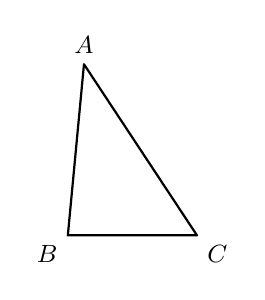
\begin{tikzpicture}[x=0.82cm,y=0.82cm,line cap=round,line join=round,line width=0.8pt,font=\small]
  \coordinate (A) at (0.25,2.65);
  \coordinate (B) at (0,0);
  \coordinate (C) at (2.0,0);
  \draw (A)--(B)--(C)--cycle;
  \node[above] at (A) {$A$};
  \node[below left] at (B) {$B$};
  \node[below right] at (C) {$C$};
\end{tikzpicture}
